% THIS IS SIGPROC-SP.TEX - VERSION 3.1
% WORKS WITH V3.2SP OF ACM_PROC_ARTICLE-SP.CLS
% APRIL 2009
%

\documentclass{acm_proc_article-sp}
\usepackage{url}
\usepackage{array}

\begin{document}

\title{A survey on the uses of RSA: Searching for bad primes with CUDA}

\numberofauthors{1}
\author{
\alignauthor
Joseph White\\
       \affaddr{California Polytechnic State University}\\
       \affaddr{1 Grand Ave.}\\
       \affaddr{San Luis Obispo, California}\\
       \email{jwhite09@calpoly.edu}
}
\date{22 March 2013}

\maketitle
\begin{abstract}
The work here presents a survey of RSA keys and investigates ways in which they
are applied in real-world scenarios. Research was done to gain an understanding
of the breadth of usages. The focus was X509 certificates due to their
prevalence and ease of obtainment. After applying the research by collecting
data, several levels of analysis was done to gain understanding of the state
of security concerning X509 certificates in high traffic areas of the Internet.
No keys susceptible to the vulnerability described in \cite{lenstra2012ron},
which was the vulnerability focused on in the analysis presented here. The
analysis here is brief, and there are plans to expand it. Near-future plans
include using a larger database of keys in order to make the check of robust
and possible expansion to include 2048-bit keys.
\end{abstract}

\category{D.3}{Data Encryption}{Public key cryptosystems}

\terms{Documentation, Security}

\keywords{Alexa top 1 million, digital rights management, RSA analysis, survey, X.509 certificates}

\section{Introduction}
A parallel analysis tool for RSA keys is described and implemented in
the work shown in \cite{scharfglass2012breaking}. This work's primary focus is
on speedup and performance of the implementation. Scharfglass et. al. use
NVIDIA's CUDA framework to significantly speedup a check for the vulnerability
presented in \cite{lenstra2012ron}. The work in \cite{scharfglass2012breaking}
lacks any context or explanation or usage for RSA keys in general, and although
their data set is security- and encryption-focused, no discussion is given to
the security aspects and the potential impacts of the work. The work would
benefit from context and specifics about RSA and what the existence of
vulnerable keys means for an end-user or a system administrator.

Research was done to learn specific ways that RSA keys are used in practice.
Most initial research yielded general statements that did not explain or give
appropriate context to RSA (statements including ``\dots all over the
Internet\dots" were accurate, but not informative). More in-depth research
yielded two primary use-cases of RSA: Digital Rights Management (DRM) and
Secure Socket Layer (SSL) and Transport Layer Security (TLS) Internet
security protocols. Other uses included password alternatives (e.g. ssh
connections or command line interface tools like \texttt{git}) but these are
more difficult to collect data for and analyze since they tend to be done on
an individual basis, and are managed by individual users.

The rest of the paper is formatted as follows. First we'll describe several
points of background information. This work pulls from and ties into various
areas and brief description of each are necessary. Next, we'll discuss our
data collection method: both what data was collected, and how we did so. Then,
we'll go over how we chose to analyze the collected data. We'll finish the work
by describing what kind of implications this adds to the integral work in
\cite{scharfglass2012breaking} and finish with what we'd like to do next and
conclude.

\section{Background}
A brief background of RSA is necessary for understanding some of the work done
here. RSA is an asymmetric key encryption scheme. Keys come in matched pairs:
public keys and private keys. Using the same algorithm, information encrypted
with the one key, can be decrypted with the other and vice versa. A party must
keep the private keep secret, but the public portion of the key can be seen and
used by anyone in the world. To generate a pair, an algorithm is performed on
two randomly-generated prime numbers whose product is of a certain bit-length
(e.g. 1024 bits). These are the primes that our work looks to discover
inadequacies with.

The work presented by Lenstra et. al. \cite{lenstra2012ron} shows that around
0.2\% of RSA keys collected from sources including the SSL Observatory suffer
from inadequate random prime generation. They show that when the primes used to
build an RSA public-private key pair are not actually random, factoring does
not need to be done to break the keys. Instead, only a greater common divisor
needs to be calculated between two RSA moduli. When anything greater than 1 is
found as a result of this calculation, the keys can be considered broken and
offer no protection. This is because once a GCD greater than 1 is found, the
private keys can be generated from the publicly available information. The
vulnerability is explained in detail in Figure \ref{fig:vuln}.

\begin{figure}
   \centering
   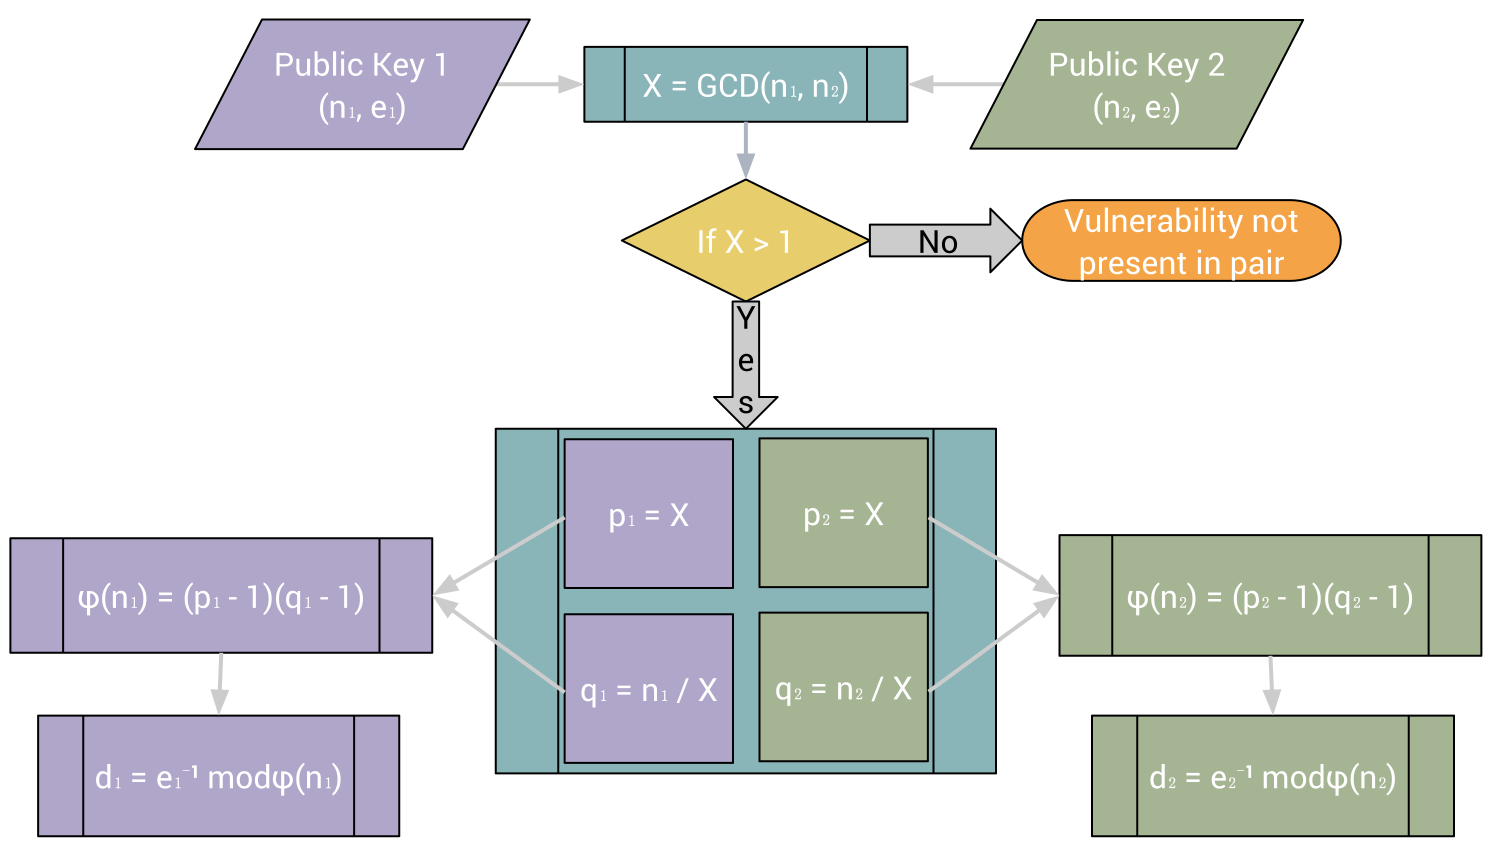
\includegraphics[width=3.3in]{vulnerability.png}
   \caption{Explanation of poor-prime vulnerability}
   \label{fig:vuln}
\end{figure}

The tool by Scharfglass et. al. \cite{scharfglass2012breaking} performs a
parallelized version of this GCD calculation (using the binary GCD algorithm)
between every pair combination in a given set of keys. It structures these
calculations so that as many as possible can be done at once. To increase
parallelism, and because the keys are so large, they are broken up into 32
chunks, which are also operated on in parallel using the GPU. Through these 2
levels of parallelism, a speedup of 27.5 is achieved. This tool provides a
practical tool for checking a given set of keys for the vulnerability we are
focusing on. We will describe our usage of this tool after detailing our data
collection methodology.

Digital rights management is a protocol used to secure the usage and
distribution of various types of media content. It is adopted by content
providers and device manufacturers to ensure users don't misuse or wrongfully 
share protected, copyrighted content.
The RSA Association proposed a protocol that could be applied to various types
of media content that secured its usage \cite{rsa2004announces,
rsa2004supports}. These announcements argued that using RSA for DRM offered
benefits to the content providers, the device manufacturers, and, arguably, the
consumers of the content. It apparently allowed device manufactures and
content providers to ensure proper usage of protected content while allowing
users to consume and playback their rightfully-owned media on an array of
their own devices.
 
Internet security relies on a particular protocol called SSL and its successor
TLS. These protocols define how to securely transfer information over the
Internet by using encryption and signing mechanisms. One aspect of both the SSL
and TLS protocols involve certificates to ensure the expected party is
actually being communicated with. These certificates provide information
about a server that a user is connected to (e.g. Amazon or Google)
and is signed by a certificate authority (e.g. Verisign). These certificates
are also encrypted with a subject's (e.g. Amazon) public key to ensure that
the entity is who they say they are. Furthermore, the public key is then used 
to transfer information back to the subject in a secure way. Figure
\ref{fig:tls} describes the TLS process between a client and server. 

The most widely used type of certificate is the X.509 certificate, whose current
revision is 3. A breakdown of the major sections of the certificate is shown in
Figure \ref{fig:x509}. The ``Subject Public Key Information" section of the
certificate held the relevant data (the subject's RSA public key) for our work.
The public key portion of the certificates can actually use one of several
algorithms defined in the specification. RSA is by far the most popular,
accounting for over half of the found certificates (as shown in Figure
\ref{fig:certs}). Other options include DSA and Diffie-Hellman. For more
detailed information about X.509 certificates and analysis on their
infrastructure, see \cite{holz2011ssl}.

\begin{figure}
   \centering
   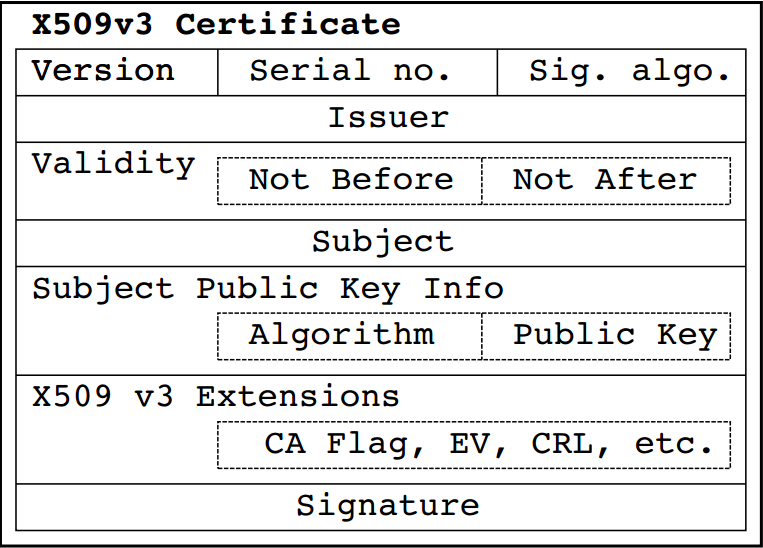
\includegraphics[width=3.3in]{x509.png}
   \caption{X.509 Fields\cite{holz2011ssl}}
   \label{fig:x509}
\end{figure}

\begin{figure}
   \centering
   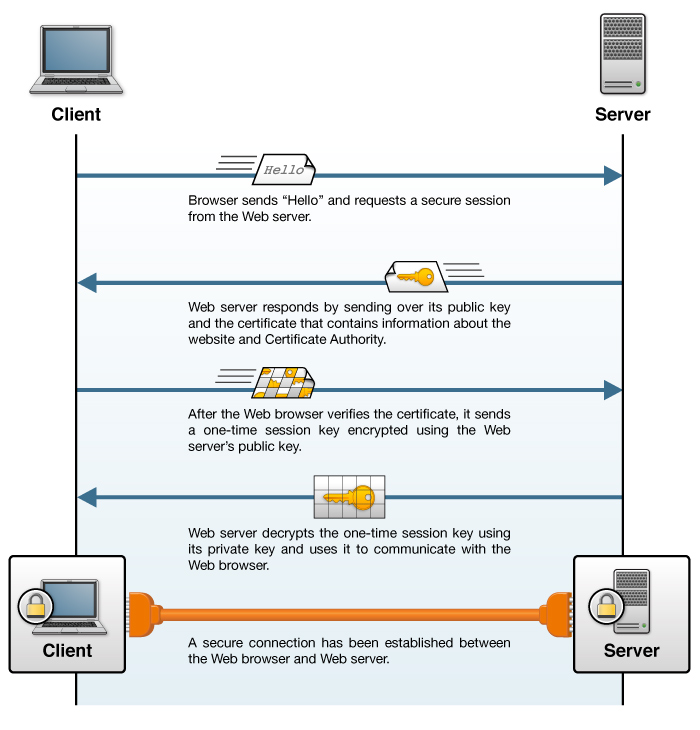
\includegraphics[width=3.3in]{tls.jpg}
   \caption{TLS Overview\cite{tlsconcepts}}
   \label{fig:tls}
\end{figure}

\section{Data Collection}
The proposed protocol given by the RSA actually modeled the certificate model
used by SSL/TLS. For this reason, the SSL certificate model was the primary
focus of the data collected. Moreover, the data set of RSA keys in SSL
certificates is much larger than DRM implementations that use RSA. Thus, the
data set that was collected and then analyzed consisted entirely of X.509
certificates.

Since a primary motivation of this work is the potential impact that vulnerable
RSA keys may have, a data set representative of a large portion of traffic was
desired. A survey was done over 2007-2010 \cite{labovitz2011internet} that
gathered some useful data on the Internet as a whole. Relevant to web traffic,
this study showed that together, the major content data networks (CDN) (i.e.
Google, Facebook, Amazon, etc.) account for nearly 17\% of web traffic.
Specific breakdowns and conversions can be found in Table \ref{tab:traffic}.

\begin{table}
\centering
\caption{Major CDN Traffic (2010)}
\begin{tabular}{|>{\raggedright}p{0.4\linewidth}
                |>{\raggedright}p{0.2\linewidth}
                |>{\raggedright\arraybackslash}p{0.2\linewidth}|}\hline
   \textbf{CDN} & \textbf{Percent of all Internet traffic} & \textbf{Approx. percentage of web traffic}\\ \hline
Google & 7 & 12.72\\ \hline
Facebook & 0.45& 0.818\\ \hline
Amazon CDN (NASA/JPL, PBS,\dots) & 0.55 & 1\\ \hline
EdgeCast (Yahoo!, Break, Imgur,\dots) & 0.5 & 0.909\\ \hline
LeaseWeb (Heineken, Starbucks,\dots) & 0.8 & 1.454\\
\hline\end{tabular}
\label{tab:traffic}
\end{table}

Alexa was used to find websites with large amounts of
traffic\footnote{http://www.alexa.com/}, as it serves as one of the Internet's
most prevalent sources for traffic information. In addition to individualized
site traffic data, Alexa provides a daily-updated list of the top one million
websites ordered by
traffic\footnote{http://s3.amazonaws.com/alexa-static/top-1m.csv.zip}. In
regards to the previous point concerning CDNs and traffic breakdowns, it was
noted that all web sites hosted by the major CDNs from
\cite{labovitz2011internet} are present in the top one million list.
Additionally, the vast majority of sites from the top one million list were
not provided by the CDNs mentioned in \cite{labovitz2011internet}. This means
that a much larger percentage than 17\% is actually represented by the sites
in the list, although quantifying precisely how much becomes difficult, and
lies beyond the scope of this project.

A Python script was used to parse the CSV file provided by Alexa. Each
extracted URL was visited on port 443 (corresponding to ``https://") using 
\texttt{openssl}. If a site responded on that port, it provided an X.509
certificate to be parsed and verified. Most of the time, this is done by a
user's web browser which has certificate authorities' private keys hidden
within. However, since the work here was not concerned with the actual web
content, the certificate was simply saved. When certificates were found, the
``Subject Public Key Algorithm" section was inspected. If this contained some
form of RSA, \texttt{openssl} was used again to extract the RSA key and save
it into a PEM file (a standard format for saving public and private key
information in). Additionally, since part of this work's motivation lies in
expanding the work done in \cite{scharfglass2012breaking}, the keys were also
stored into a SQLite3 database so that later retrieval by the tool was trivial.

After writing an initial implementation of the Python script, it was realized
that the collection process was too slow. Therefore, some of Python's
multi-process capabilities were utilized to speed up the collection of data.
Eight processes were spawned to perform the work described above. Seven of the
processes read URLs from a deque (double-ended queue) and attempted to obtain
an X.509 certificate and RSA key from each. When found, these keys were added
to a queue. These data structures not only offered convenient structures for
organizing the data, but were also thread-safe and could be used with our
updated implementation. An eighth thread read keys from the queue and entered
them into the SQLite3 database. This reimplementation offered a 15$\times$
speedup over the previous, na\"{i}ve approach.

\section{Data Analysis}
After collecting data from each of the top one million Alexa sites, some
surface-level analysis was performed in order to gain an overview of the
security of these one million sites. This analysis included overall security
breakdowns (i.e. whether a site used any kind of security) and
bit-length breakdowns of the RSA keys that were found. This data analysis can
be found in Figures \ref{fig:certs} and \ref{fig:bits}. Table \ref{tab:bits}
offer specific breakdown for bit-lengths, and offers details that cannot be
seen in the figure.

\begin{figure}
   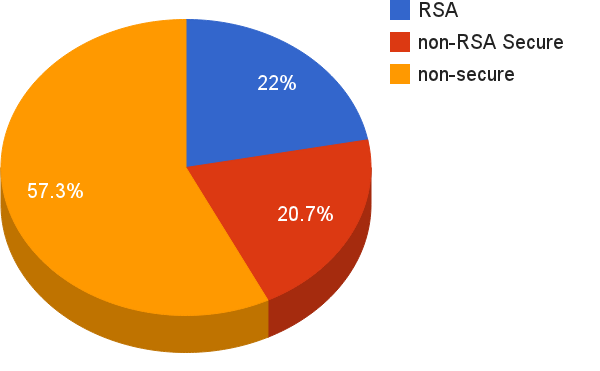
\includegraphics[width=3.3in]{cert_security.png}
   \caption{Presence of RSA key or other security in Alexa top 1M sites}
   \label{fig:certs}
\end{figure}

Interestingly (and slightly worrisome), is that the majority of web sites in
this top one million list did not even respond on port 443, implying that
they do not allow any option for secure traffic to their site. Nearly 60\% of
websites in the list fell into this category.

Also of note are the specifics of bit-lengths found. It is a surprising data
set for various reasons. First, bit-lengths as small as 384, 512, and 768 were
not expected as keys of this size were factored years ago
\cite{rsa2007challenge}, and cannot be expected to offer much
security\footnote{Interesting note: The author attempted to visit the sites
384-bit keys. Google Chrome did not find a web page on port 443 for any of
the sites.}.

On the other hand, the high number of longer bit-lengths was also surprising,
but comforting. The fact that the vast majority of keys were 2048-bit was not
expected, but means that a large number of high-traffic websites have adequate
(for now) encryption. Moreover, there were quite a number of sites with 4096,
and, even more surprisingly, 8192-bit.

\begin{figure}
   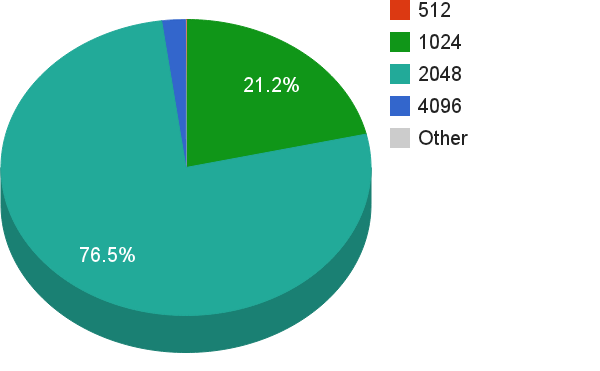
\includegraphics[width=3.3in]{bit_length.png}
   \caption{Breakdown of Alexa top 1M sites' RSA keys by bit-length}
   \label{fig:bits}
\end{figure}

\begin{table}
\centering
\caption{Alexa top 1M X.509 RSA bit-length}
\begin{tabular}{|r|r|}\hline
\textbf{Bits} & \textbf{Count}\\\hline
384 & 4 \\ \hline
512 & 309 \\ \hline
768 & 4 \\ \hline
1024 & 46736 \\ \hline
2048 & 168391 \\ \hline
2432 & 37 \\ \hline
3072 & 17 \\ \hline
4096 & 4511 \\ \hline
8192 & 14 \\ \hline
other & 44 \\ \hline
\end{tabular}
\label{tab:bits}
\end{table}

Further analysis was done using the tool described in
\cite{scharfglass2012breaking}. This tool performs a complete check of all
RSA keys in a given set for the previously mentioned vulnerability described
in \cite{lenstra2012ron}. This check is done using NVIDIA's CUDA framework to
parallelize the work as much as possible which allows for a practical security
validation tool. At the time of writing, the tool's current implementation is
limited to 1024-bit RSA keys. Due to this limitation, the data set was
reduced to 46,736 RSA keys. Due to the $O(n^2)$ nature of this problem,
this check resulted in $1,092,150,216$ comparisons. The run of the tool using
this data set took 138 minutes, 37 seconds or $131,305$ comparisons per second.
After applying the tool to this set of keys, it was found that no keys were
susceptible to the vulnerability (insofar as none of the keys in the set
shared primes with a given key). Although no vulnerabilities were detected,
this does not mean the set is completely secure from the previously mentioned
vulnerability. Since such a limited data set was used, and the security tool
relies on large sets to accumulate many primes, the analysis presented can
only be considered an initial pass.

\section{Implications}
For the same reasons the data set was chosen to be X.509 certificates, presence
of the vulnerability mentioned here would have the largest effect on Internet
security: specifically in the certificate infrastructure. If servers were
unknowingly providing compromised public keys in their certificates, their
traffic could offer no security if this became known. This could offer
ill-effects since the vulnerability is agnostic of the type of data being
being encrypted.

Additionally, the password-alternatives that were mentioned briefly before
could be particularly impacted. If a system was generating many new RSA keys
(e.g. a user is building new accounts for various websites, and tying RSA keys
to them) with inadequate primes, potentially all these accounts for this user
could end up compromised, despite the sense of stronger security.

Along these lines, a system administrator could potentially suffer from similar
issues. If many machines and key-pairs are being setup and generated as part of
an initial setup process for a new network of users, poor random number
generation could have severe consequences when done at scale. This would likely
create many new, vulnerable keys at once. By being aware that this problem
could exist, and that a tool such as \cite{scharfglass2012breaking} exists, an
insecure set of users could be avoided or detected much earlier than would have
otherwise occurred.

\section{Future Work}
As mentioned, this survey suffers from various limitations. Some immediate
steps are recommended to make the analysis more complete. Primarily, a larger
data set of any kind must be used with the tool in
\cite{scharfglass2012breaking}. This could come in several ways. First,
additional keys could be generated and added to the set of $46,736$ so that more
prime values are present in the pool of primes. Second, more primes could be
collected from other certificates online. The tool gains functionality as the
number of keys increases, so the more keys used, the more complete the results.

Furthermore, extending the functionality to 2048-bit keys would offer several
advantages over the present work. First, a much more accurate analysis of
high-traffic X.509 certificates could be gained since this was the largest
portion of the data collected (see Figure \ref{fig:bits}). Second, it would
offer a much larger data set, which, as previously mentioned, adds
effectiveness to the tool.

The survey could also be expanded to include public keys from the 
previously-mentioned self-maintained keys (e.g. password alternatives). If
these keys were accessible from some set of services, it could contribute to
the data sets significantly. This would especially hold true if there existed
ways to correlate where specific keys originated form (i.e. which machine
generated them). This way, when vulnerable keys were found, a machine could be
flagged as potentially insecure for key generation.

\section{Conclusions}
This survey determined that the primary use of RSA keys in practice is the
signing of SSL certificates. A data set was gathered that accounts for a
significant amount of certificates in the context of web traffic. Some
surface-level analysis was done to gain a general understanding of the
collected data. A high-performance tool was then applied to a subset of the
data to check for a vulnerability within the data subset. No vulnerabilities
were found; however, due to limitations in the tool used, as well as
limitations in the data set, this cannot be considered a complete analysis
and requires further investigation.

\balancecolumns
Though limited, this survey does successfully add real-world application
context to the work done in \cite{scharfglass2012breaking}. Specific
implications are able to be draw from the practicality of the tool, and more
tangible examples of what vulnerabilities in RSA keys looks like have been
realized.

\bibliographystyle{abbrv}
\bibliography{references}

\end{document}
